\documentclass[%
    reprint,
    amsmath,amssymb,
    aps,
]{revtex4-2}

\usepackage{graphicx}
\usepackage{dcolumn}
\usepackage{bm}

\begin{document}

\preprint{APS/123-QED}

\title{Learning Renormalization Group Flows for Lattices}

\author{Jay Shen}
\thanks{
    My deepest gratitude goes out to Professor Kao at NTU for his guidance and hospitality at NTU. I'd also like to thank the NTU physics department buddies and my officemates for their friendship and the cultural exchange we shared. Finally, a huge thanks to all the donors from the UCTS program, the SITG program, the Metcalf Foundation—as well as Professor Chin at UChicago—for making my summer in Taiwan possible in the first place. 
}
\affiliation{
    Department of Physics \\
    University of Chicago
}
\email{jshe@uchicago.edu}

\begin{abstract}

    Real space renormalization is a powerful and theoretically fascinating, albeit 
    difficult technique for investigating scale and phase behavior in physical systems. For even the simplest problems, formulating the so-called renormalization group (RG) flow involves incredibly tedious, intuition-dependent work that can drag on for years. However, once accurately described, RG flows have a number of uses, from describing phase behaviors to speeding up simulations. Accordingly, any information at all about their properties is highly valued and sought after by physicists. In this work, we review and assess a novel approach to real space renormalization initially proposed by Hou et al. \cite{mlrg}. The so-called Machine Learning Renormalization Group (MLRG) algorithm automatically determines approximate RG flows of translationally-invariant Ising models, given only the symmetry description of the lattice. It has the potential to effectively characterize a wide range of interesting systems, and also demonstrates an elegant synthesis of both new and old machine learning techniques with statistical physics. In the Section \ref{sec:background}, we will first give some background for real space renormalization and the Ising model. In Section \ref{sec:mlrg}, we will describe the MLRG algorithm and demonstrate its use. In Section \ref{sec:design-space}, we will discuss the algorithmic design space and explore modifications for improvement. 

\end{abstract}

\maketitle

\section{Background} \label{sec:background}

\subsection{The Gist of Real Space Renormalization}

Real-space renormalization is a theoretical framework for understanding scale in physical systems \cite{fisher-rg, wilson-rg}. That is, it tries to understand how the apparent behavior of a system changes with the length scale. 

As a toy example, consider the task of modeling some volume of water.
At the very smallest scales, we might use field theories or quantum mechanics to describe the microscopic dynamics composing each and every atom. 
This approach requires a simply enormous amount of information—think positions, momenta, etc. 
In addition, the relations between these degrees of freedom are, more often than not, impossibly complex and intractable to solve. 

However, if we choose to "zoom out" to a somewhat larger scale, things become substantially simpler and more manageable. 
At the human scale, for example, fluid mechanics accurately describes the hydrodynamics of the water. 
But compared to the smaller-scale theories, it is much simpler model, requiring only a few parameters—viscosity, pressures, temperatures, etc.—to fully specify the system. 
Computation is also completely tractable and comparatively straightforward. 

We ask, in what way are all these theories, which model the same system, linked? 
Why are small scales complex and large scales simple? 
How is this all connected to the thermodynamic phase behavior of the system? 
Real space renormalization provides answers to these questions, and more. 
For simplicity, in this paper we will only describe real space renormalization as it pertains to the Ising model. 
It is our hope that it is an example rich enough to demonstrate real space renormalization and illustrate its profound importance. 

\subsection{The Ising Model}

The Ising model is a historically important problem in statistical physics as well as computer science and machine learning \cite{brush-ising, ising}. 
Originally devised as a thermodynamic model of ferromagnetism, it has since been applied to a wide range of problems, including some beyond physics.

The Ising model takes the form of up-down spins arranged on a regular lattice. 
\begin{figure}[h]
    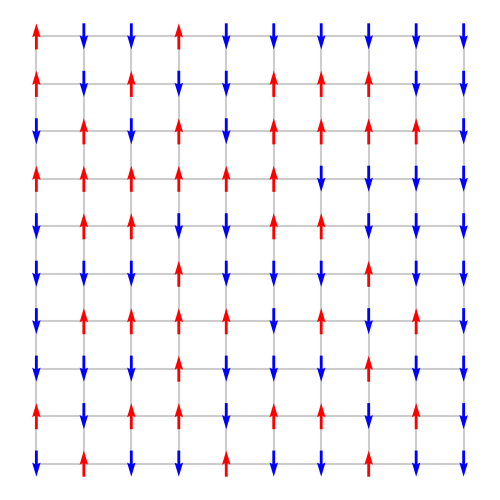
\includegraphics[width=0.25\textwidth]{tex/images/ising-spins-grid.png}
    \caption{\label{fig:ising}
        A random Ising model on a square lattice. 
    }
\end{figure}
Each spin is correlated to its neighboring spins—namely, those adjacent to it on the lattice. 

We can model this with a Hamiltonian representing the total energy of the system:
\begin{eqnarray}
    \label{eqn:ising-hamiltonian}
    H(J, \vec{\sigma}) = -J \sum_{(i, j) \in \mathcal{E}} \sigma_i \sigma_j
\end{eqnarray}
Here, $\vec{\sigma}$ is a vectorized list of all the spins in the Ising model. 
$(i, j) \in \mathcal{E}$ means the spins $i$ and $j$ are neighbors on the lattice. 
$J \in \mathbb{R}$, called the coupling constant, specifies the correlation strength between spins. 
$\sigma_i, \sigma_j \in \{-1, +1\}$ are the values of spins $i$ and $j$. 

If $J > 0$, the system is ferromagnetic, and aligned spins lower the energy while misalign spins raise it. 
If $J < 0$, the system is antiferromagnetic and the reverse is true: aligned spins raise the energy and misaligned spins lower it. 
If $J = 0$, the system is non-interacting and the spins have no correlation. 

Using this Hamiltonian, we can define a Gibbs probability distribution over all the states of an Ising model:
\begin{eqnarray}
    \label{eqn:ising-gibbs}
    P(J, \vec{\sigma}) = \frac{1}{Z} e^{-H(J, \vec{\sigma})}
\end{eqnarray}
Implicitly, this assigns higher probabilities to lower energy states. 

\subsection{Real Space Renormalization of the Ising Model}

Say we have some Ising model defined by a specific lattice and a coupling constant $J$. 
We would like to ``zoom out'' and understand what this Ising model looks like from some larger length scale. 

To apply real space renormalization, we must first engineer a \textit{coarse-graining} transformation to remove some degrees of freedom from the system. 
This is necessary to obtain a large-scale description of the system that models macroscopic, rather than microscopic, features. 

For example, given a square lattice, we might choose Kadanoff blocking \cite{kadanoff-blocking} as our coarse-graining transformation. 
\begin{figure}[h]
    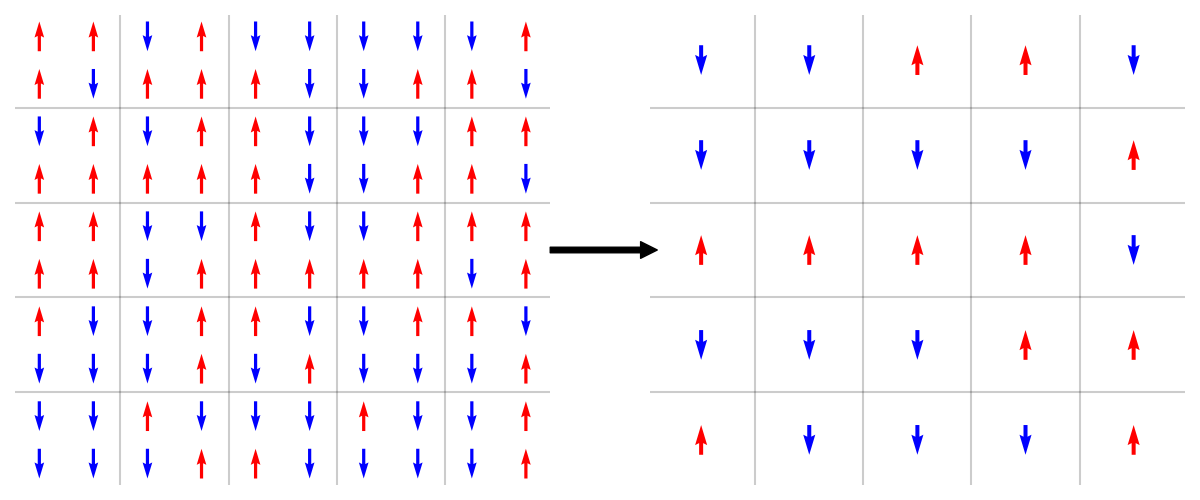
\includegraphics[width=0.45\textwidth]{tex/images/ising-blocking.png}
    \caption{\label{fig:kadanoff}
        A Kadanoff blocking procedure. 
    }
\end{figure}
Kadanoff blocking removes degrees of freedom by replacing a block of microscopic spins with a single macroscopic spin. 

Note that this transformation has the required property of \textit{scale invariance}. 
In other words, the coarse-grained system on the new set of spins $\vec{\sigma}'$ is still an Ising model. 
This means it can be modeled with the same Hamiltonian. 
Only the coupling constant $J$ will change to some $J'$ to reflect the change in scale. 
\begin{eqnarray}
    \label{eqn:ising-prime-hamiltonian}
    H(J', \vec{\sigma}') = -J' \sum_{(i, j) \in \mathcal{E'}} \sigma_i \sigma_j
\end{eqnarray}
This constitutes one real space renormalization step. 

Note that for each $J$ there is only one unique $J'$. 
This means we can write down a function modelling the change in coupling constant due to the coarse-graining transformation:
\begin{eqnarray}
    \label{eqn:rg-flow}
    J' - J = f(J) : \mathbb{R} \mapsto \mathbb{R}
\end{eqnarray}
We call this function the renormalization group (RG) flow. 
It turns out that the asymptotic behaviors of this function correspond directly to the thermodynamic phase behaviors of the system. 
Formulating this function across all values of $J$, is extremely difficult, however. 
We will now describe an algorithm that learns it automatically. 

\section{The MLRG Algorithm} \label{sec:mlrg}

\subsection{Algorithm Description}

The Ising model we use in this algorithm will be defined on the Lieb lattice. 
It is similar to the square lattice, but incorporates "hidden" spins which we can ignore when considering the visible behavior of the system. 
A single coupling constant, $J$, still mediates correlations between neighbors. 

\begin{figure}[h]
    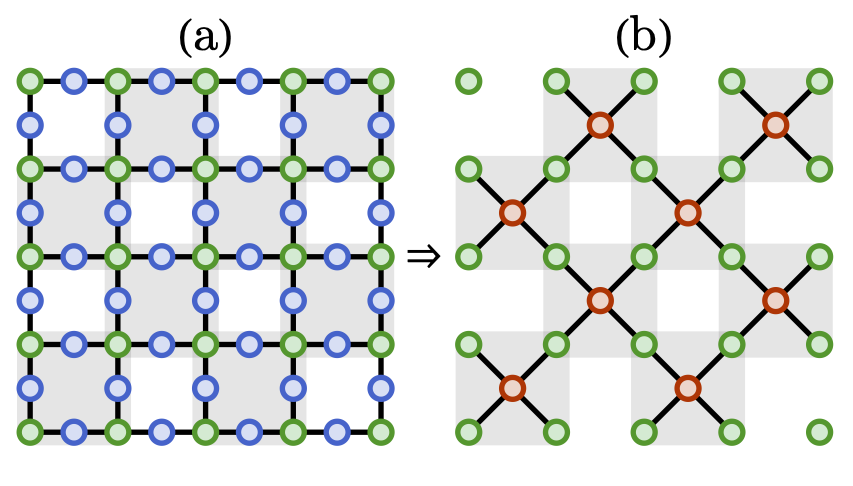
\includegraphics[width=0.4\textwidth]{tex/images/lieb-blocking.png}
    \caption{\label{fig:lieb}
        (a) The fine-grain Lieb lattice. Visible spins are green and hidden spins are blue. 
        (b) The coarse-grain Lieb lattice. The new hidden spins are red. 
    }
\end{figure}

To coarse-grain, we use the Lieb blocking transformation visualized in Figure \ref{fig:lieb}. 
Real space renormalization is applicable, as the system exhibits scale-invariance—the coarse-grained lattice is a Lieb lattice rotated by 45 degrees, with hidden and visible spins swapped. 

Let's note two niceties of the Lieb lattice important to the algorithm. 
\begin{enumerate}
    \item{
        Since the Lieb lattice is \textit{translationally invariant}, we don't need to work with an entire lattice, only the composite block that repeats to form it (Figure \ref{fig:lieb-blocks}). 
        Mathematically, this means we only need the Gibbs distributions over the block, not over the entire lattice, which would be completely unmanageable. 

        \begin{figure}[h]
            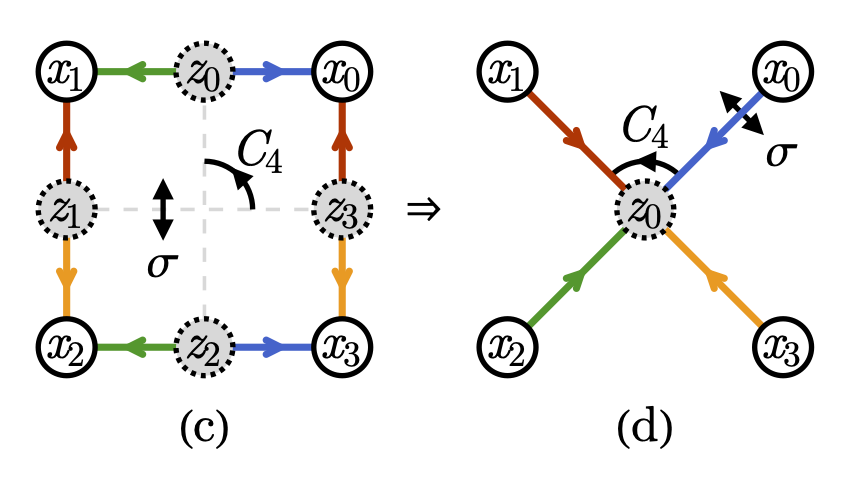
\includegraphics[width=0.4\textwidth]{tex/images/lieb-blocks.png}
            \caption{\label{fig:lieb-blocks}
                (c) The fine-grained Lieb block is a square graph. 
                (d) The coarse-grained Lieb block is a cross graph. 
            }
        \end{figure}
    }
    \item{
        Since behavior of the hidden spins doesn't matter, we only need to consider the behavior of the visible spins. 
        This will allow us to interpret the Lieb lattice as a Restricted Boltzmann Machine (RBM) \cite{hinton-rbm}. 
    }
\end{enumerate}

So how are we going to formulate $f(J)$? 
The MLRG algorithm proposes approximating \cite{universal-approximation, relu-approximation} it using a neural network:
\begin{eqnarray}
    \label{eqn:neural-network}
    f_\theta(J) : \mathbb{R} \mapsto \mathbb{R}
\end{eqnarray}
Here, $\theta$ denotes the parameters of our network which will be tuned during training. 

To train $f_\theta(J)$, Hou et al. \cite{mlrg} propose the following learning procedure: 
\begin{enumerate}
    \item{
        \textbf{Sample a value of $J$}

        We want our learned function $f_\theta(J)$ to be highly accurate around its zeroes, because their locations specify important thermodynamic fixed and critical points. 
        Elsewhere, it is fine if $f_\theta(J)$ is only reasonably accurate. 
        
        To this end, we choose to use Hamiltonian Monte Carlo (HMC) \cite{betancourt-hmc, duane-hmc}. 
        Using Hamiltonian dynamics, HMC samples from the unnormalized probability distribution:
        \begin{eqnarray}
            \label{eqn:hmc-distribution}
            \tilde{P}(J) = e^{-U(J)}
        \end{eqnarray}
        Here, $U(J)$ is a potential energy function which is minimized by the samples. 
        We set it to:
        \begin{eqnarray}
            \label{eqn:hmc-potential}
            U(J) = \beta || f_\theta(J) ||^2
        \end{eqnarray}
        
        $U(J)$ is annealed in during training by increasing $\beta$ from $\beta_0 = 0$ to a $\beta_T > 0$ according to some schedule. 
        This ensures the sampling is more or less random at the beginning of training, and we can get a general idea of the function shape. 
        Later on, as the full value of $U(J)$ kicks in, the sampler begins to sample heavily only around the points of interest, thus refining their values. 
    }\\
    
    \item{
        \textbf{Forward pass to get $J' = J + f_\theta(J)$}
        
        Remember, the $f_\theta(J)$ represents the change in the coupling constant $J$ after the coarse-graining transformation. 
        Thus we can compute $J'$, which we will use in the next step. 
    }\\
    
    \item {
        \textbf{Evaluate the error between fine and coarse-grained models}

        $J$ is the coupling constant for the fine-grained model (Figure \ref{fig:lieb-blocks}c). 
        $J'$, calculated in step $2$, is the coupling constant for the coarse-grained model (Figure \ref{fig:lieb-blocks}d). 
        Ideally, if $f_\theta(J)$ does a good job, these two models should behave as similarly as possible. 
        
        Now, the distributions over the visible spins provide our understanding of the model behaviors. 
        These are given by marginalizing hidden spins out of the original Gibbs distribution:
        \begin{eqnarray}
            \label{eqn:kl-divergence}
            P_{fine}(J, \vec{v}) = \sum_{\vec{h}} P(J, \vec{v}, \vec{h}) \\
            P_{coarse}(J', \vec{v}) = \sum_{\vec{h}'} P(J', \vec{v}, \vec{h}')
        \end{eqnarray}
        
        We can then use a Kullback-Liebler (KL) divergence to measure the difference between these distributions:
        \begin{eqnarray}
            D_{KL} = \sum_{\vec{v}} P_{fine}(\vec{v}) \log \Bigr( \frac{P_{fine}(\vec{v})}{P_{coarse}(\vec{v})} \Bigr)
        \end{eqnarray}
        Alternatively, we can use the common contrastive approximation \cite{contrastive-divergence} to the KL divergence:
        \begin{eqnarray}
            D_{C} = F_{coarse}(\vec{v}_{fine}) - F_{coarse}(\vec{v}_{coarse})
        \end{eqnarray}
        Here, $F_{coarse}$ is the free energy function of the coarse-grained model. 
        $\vec{v}_{fine}$ and $\vec{v}_{coarse}$ are configurations of visible spins Gibbs-sampled from the fine and coarse-grained models, respectively. 

        Either of these divergences is an explicit expression measuring the difference between the fine and coarse-grained distributions, and, by proxy, how well $f_\theta(J)$ predicts $J'$. 
    }
    
    \item{
        \textbf{Backpropagate error to $\theta$}

        Once we compute either $D_{KL}$ or $D_C$, we use it as a loss function and backpropagate \cite{backprop} it to adjust the parameters $\theta$. 
        This is fairly easy using auto-differentiation \cite{pytorch}, since both $D_{KL}$ and $D_C$ are computed using the forward pass value $f_\theta (J)$. 
        As training progresses, $f_\theta (J)$ will get better and better at predicting $J'$ given $J$. 
    }
    
\end{enumerate}

\subsection{Demonstration of Results}

Following this procedure, we trained a simple two-layer multi-layer perceptron (MLP) with ReLU activations as $f_\theta(J)$:
\begin{figure}[h]
    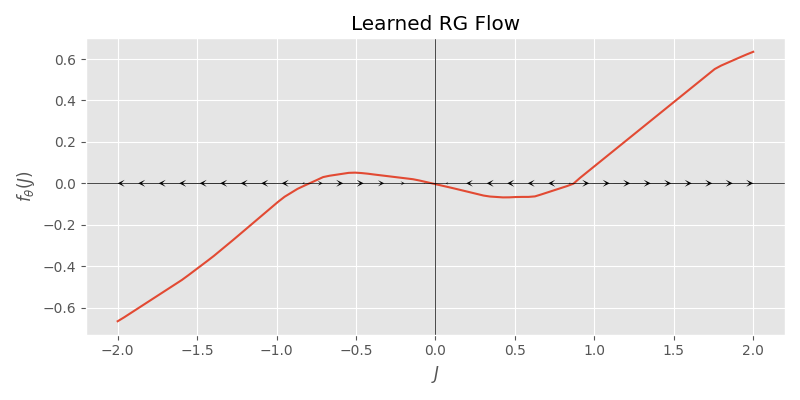
\includegraphics[width=0.5\textwidth]{tex/images/a1_flows.png}
    \caption{\label{fig:a1-flow}
        Learned $f_\theta(J)$ function in red. 
        The equivalent $1$-dimensional vector field is shown on the x-axis. 
    }
\end{figure}

At a glance, this $f_\theta(J)$ exhibits the general features we would expect:
\begin{itemize}
    \item Anti-symmetric about $J=0$
    \item Fixed points at $J = 0, -\infty, +\infty$
    \item Finite critical points where flow direction switches. 
\end{itemize}

But how precise is it?
From analytically solutions to the Ising model, we know the critical point should be located at:
\begin{eqnarray}
    \label{eqn:ising-critical}
    J_C = \frac{1}{2} \text{arccosh}(1 + \sqrt{2}) \approx 0.7643
\end{eqnarray}

Using Newton's root-finding method, we can numerically solve for the critical point predicted by $f_\theta(J)$. 
We can estimate the distribution of these predictions by training multiple instances of $f_\theta(J)$. 
A boxplot of this distribution is shown in Figure \ref{fig:a1-boxplot}. 
\begin{figure}[h]
    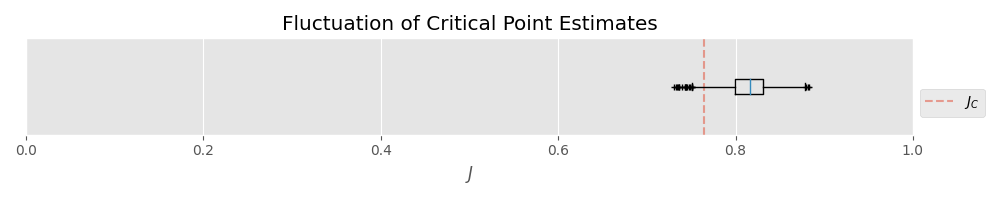
\includegraphics[width=0.5\textwidth]{tex/images/a1_critical_points_boxplot.png}
    \caption{\label{fig:a1-boxplot}
        Boxplot of predictions for $J_C$. 
        Analytical target value shown by dotted red line. 
    }
\end{figure}
We observe that, indeed, the algorithm is successful at identifying critical points near the correct value. 
In \ref{sec:design-space} we will discuss how to improve these results. 

\section{The MLRG Design Space}\label{sec:design-space}

\subsection{Bias Reduction Using Higher-Dimensional Representations}

The distribution of predictions in Figure \ref{fig:a1-boxplot} are visibly biased from the real $J_C$. 
Why?
In Section \ref{sec:sampler-hyperparameters} and \ref{sec:cd-hyperparameters}, we show some ways to slightly reduce this bias by adjusting algorithm hyperparameters.  
However, Hou et al. \cite{mlrg} conjecture that most of the bias comes from excessive information loss of relevant microscopic effects, which occurs during the coarse-graining transformation. 

To ameliorate this, they propose increasing the representational capacity of the Ising model, reasoning that the more complex the Ising model is, the more information it can retain past coarse-graining. 
This can be done by using \textit{higher-dimensional} lattices—in short, decorating the base Ising model with more spins and wiring additional correlations between those spins (See Figure \ref{fig:a1-a1e-edge})
\begin{figure}[h]
    (a)
    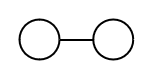
\includegraphics[width=0.4\linewidth]{tex/images/a1-edge.png}
    (b)
    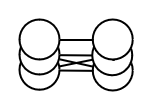
\includegraphics[width=0.4\linewidth]{tex/images/a1e-edge.png}
    \caption{\label{fig:a1-a1e-edge}
        (a) A bond in a base 1-dimension Ising model ($A_1$ representation)
        (b) A bond in a 5-dimension Ising model ($A_1 \oplus E$ representation)
    }
\end{figure}
Now, these higher-dimensional lattices must have the same symmetries as the original, base Ising model. 
We can ensure this by referencing the representations of the lattice symmetry group. 
See Hou et al. \cite{mlrg} for an in-depth discussion of this process. 

The same general learning algorithm can be applied to these higher-dimensional lattices. 
However, since we added additional correlations between spins, we will have more coupling constants that need to change during the coarse-graining transformation. 
If we have $n$ coupling constants, we can express the coupling constants by a vector $\vec{J} \in \mathbb{R}^n$. 
The RG flow, which we want to model, is also higher-dimension now:
\begin{eqnarray}
    \label{eqn:nd-flow}
    \vec{J}' - \vec{J} = \vec{f}(J) : \mathbb{R}^n \mapsto \mathbb{R}^n
\end{eqnarray}

We can verify Hou et al.'s conjecture, observing in Figure \ref{fig:a1-a1e-boxplot} that increasing the lattice dimensionality does in fact reduce the prediction bias. 

\begin{figure}[h]
    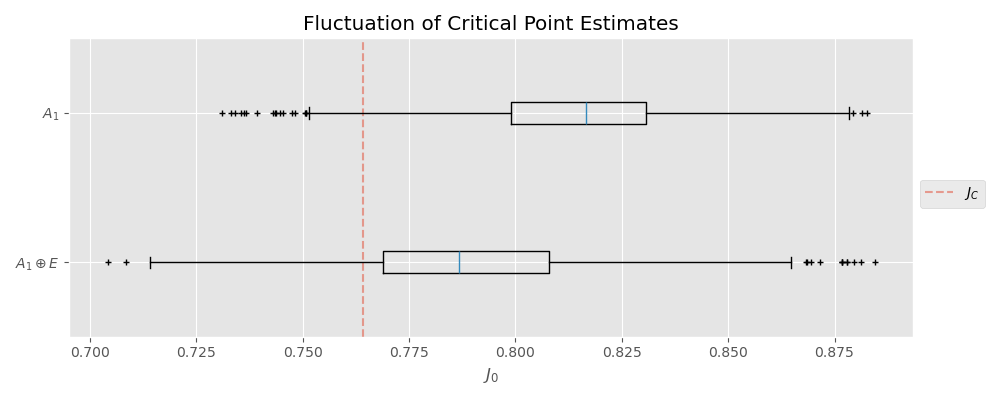
\includegraphics[width=0.5\textwidth]{tex/images/a1-a1e-critical-points-boxplot.png}
    \caption{\label{fig:a1-a1e-boxplot}
        Boxplot of predictions for $J_C$ using an $A_1$ representation (1 dimension) versus an $A_1 \oplus E$ representation (5 dimensions). 
        Analytical target value shown by dotted red line. 
    }
\end{figure}

Hou et al. \cite{mlrg} further show that as the number of dimensions increases, that is as $n \rightarrow \infty$, the bias seems to go to $0$. 
Unfortunately, due in part to the curse of dimensionality, this comes at the significant cost of degraded training stability and increased compute time. 
Nevertheless, this is reassuring, as it provides a loose scaling law for the algorithm's predictive accuracy. 

\subsection{Learning the Flow versus the Monotone}

In all our results so far, we have learned the RG flow function $\vec{f}(\vec{J}) = \vec{J}' - \vec{J}$. 
In their paper, however, Hou et al. learn instead the RG monotone function:
\begin{eqnarray}
    \label{eqn:rg-monotone}
    C(\vec{J}) : \mathbb{R}^n \mapsto \mathbb{R}
\end{eqnarray}

According to the C-theorem \cite{c-theorem}, the monotone $C(\vec{J})$ has the important property of always decreasing monotonically under the Ising model RG flow, and is guaranteed to exist. 
Learning $C(\vec{J})$ is attractive because of this theoretical soundness. 

On the other hand, learning $\vec{f}(\vec{J})$ is theoretically shaky. 
It is related to the monotone by:
\begin{eqnarray}
    \vec{f}(\vec{J}) = \vec{\nabla} C(\vec{J})
\end{eqnarray}
However, the $\vec{f}_\theta(\vec{J})$ we learn might not be, and usually is not, the gradient of any function. 

Qualitative observations seem to suggest, however, that learning $\vec{f}(\vec{J})$ is good enough for our purposes, and we see no significant degradation in predictive abilities and accuracy. 

Moreover, learning $\vec{f}(\vec{J})$ is significantly faster, not to mention easier to implement. 
This is because learning $C(\vec{J})$ requires computing $\vec{\nabla} C(\vec{J})$ in the forward pass for $\vec{J}' = \vec{J} + \vec{\nabla} C(\vec{J})$, as well as $\vec{\nabla} ||\vec{\nabla} C(\vec{J})||^2$ during Hamiltonian Monte Carlo sampling. 
These first and second-order derivatives are very expensive for auto-differentiation to compute and backpropagate. 
Learning $\vec{f}(\vec{J})$, on the other hand, only requires computing at worst the first-order quantity $\nabla || \vec{f}(\vec{J}) ||^2$. 
The compute time difference is shown in Figure \ref{fig:flow-monotone}. 
\begin{figure}[h]
    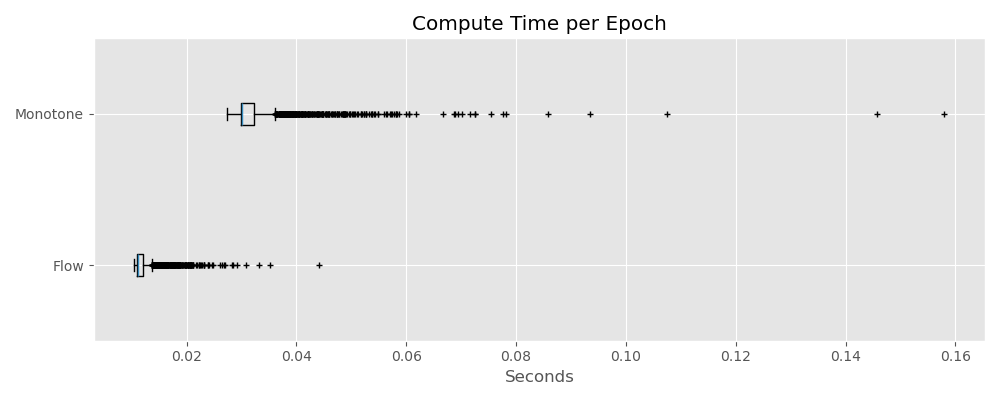
\includegraphics[width=0.5\textwidth]{tex/images/a1-silu-flow-monotone-times.png}
    \caption{\label{fig:flow-monotone}
        Compute time per training epoch for learning the monotone $C(\vec{J})$ versus learning the flow $\vec{f}(\vec{J})$. 
    }
\end{figure}

As a side note, learning the flow $\vec{f}(\vec{J})$ also permits the use of non-smooth non-linearities like ReLU in the neural network, which wouldn't be compatible with Newton's method if learning the monotone. 

More work is needed to investigate any possible consequences of learning the flow instead of the monotone. 

\subsection{KL vs Contrastive Divergence}

So far, we have used the contrastive divergence as our loss function, instead of the KL divergence, mostly to adhere to convention—the KL divergence is typically intractable to compute. 
However, in the case of the $A_1$ representation ($1$-dimensional) Lieb Ising model, the KL divergence is actually tractable to evaluate—there are only a few hundred spin configurations to sum over. 

In the machine learning literature, there has been skeptism about the validity of the contrastive approximation \cite{bengio-cd, sutskever-cd, carreira-cd}, including assertions that it can introduce bias. 
We wish to elucidate whether or not this affects our learned model. 

\begin{figure}[h]
    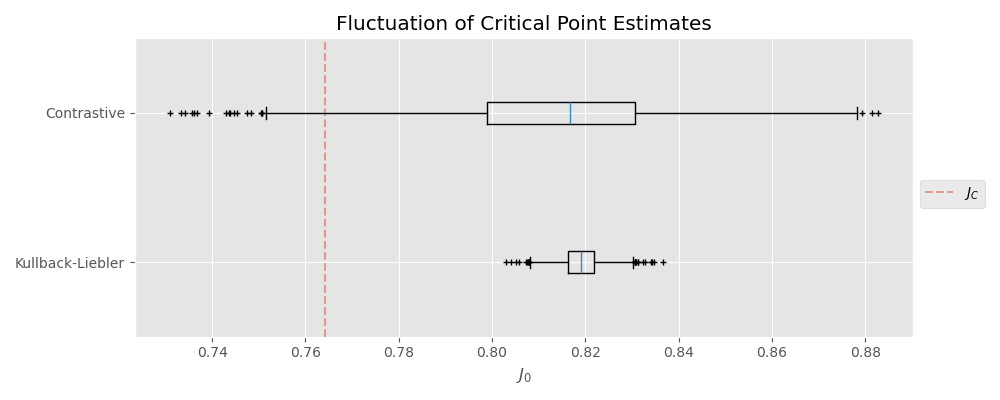
\includegraphics[width=0.5\textwidth]{tex/images/a1_critical_points_divergence_boxplot.png}
    \caption{\label{fig:cd-kl}
        Distributions of critical point predictions using the contrastive versus KL divergences as our loss function. 
    }
\end{figure}

We observe in Figure \ref{fig:cd-kl} that, in fact, using the KL divergence only really affects the variance of our predictions, not the bias. 
Since there are other ways to reduce variance, such as decreasing learning rate, and variance is not a particularly pressing issue, we conclude that the extra compute cost needed to use the KL divergence is not worth it. 
Furthermore, the KL divergence does become intractable when using higher-dimension representations. 

\subsection{Divergence Hyperparameters} \label{sec:cd-hyperparameters}

If we decide to use the contrastive divergence as our loss function, we want to be sure to compute it correctly and efficiently. 
There a few hyperparameters to control for: 
\begin{itemize}
    \item The number of samples to take from the models: the batch size, more or less
    \item The number of Gibbs sampling steps for the fine-grained model
    \item The number of Gibbs sampling steps for the coarse-grained model
\end{itemize}
The effect on $A_1$ critical point predictions from varying each of these hyperparameters, while holding all others constant, is shown in Figure \ref{fig:cd-hyperparameters}.

\begin{figure}[h]
    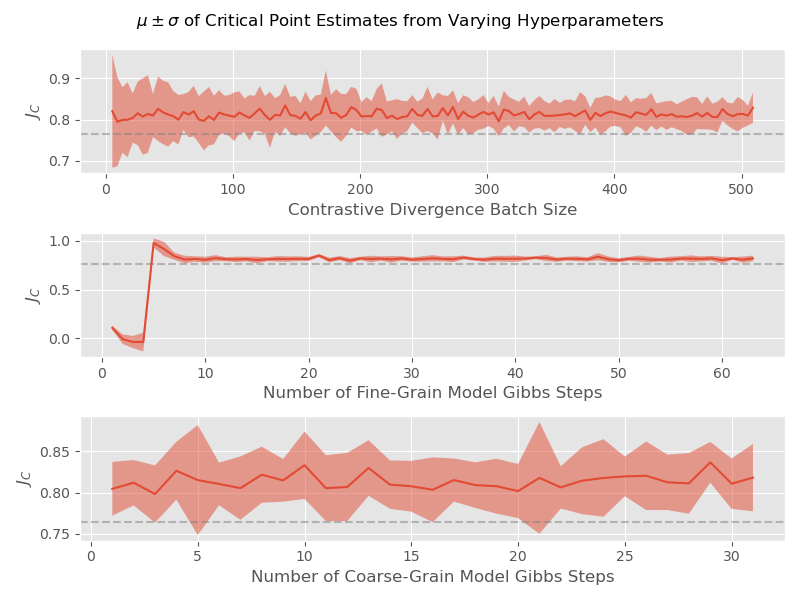
\includegraphics[width=0.45\textwidth]{tex/images/cd-hyperparameters.png}
    \caption{\label{fig:cd-hyperparameters}
        Hyperparameter space explorations for three contrastive divergence hyperparameters. 
    }
\end{figure}

We conclude that:
\begin{itemize}
    \item The batch size should be fairly large to control variance, though there are diminishing returns past a few hundred samples. 
    \item The number of fine-grained model Gibbs steps should be larger than a minimum threshold to control bias
    \item The number of coarse-grained model Gibbs steps can be minimal—$1$ is plenty
\end{itemize}

\subsection{Sampler Hyperparameters} \label{sec:sampler-hyperparameters}

There are a number of hyperparameters to set for the HMC sampler. 
Here, we do a limited hyperparameter space exploration for the following:
\begin{itemize}
    \item The number of trajectories: basically the sample batch size
    \item Number of solve steps: controls for how long the numerical integrator solves the Hamiltonian equations. 
    \item Number of sampling steps: controls how many repeated, refining Monte Carlo iterations are performed. 
\end{itemize}
The effect on $A_1$ critical point predictions from varying each hyperparameter, while holding all others constant, is shown in Figure \ref{fig:hmc-hyperparameters}. 

\begin{figure}[h]
    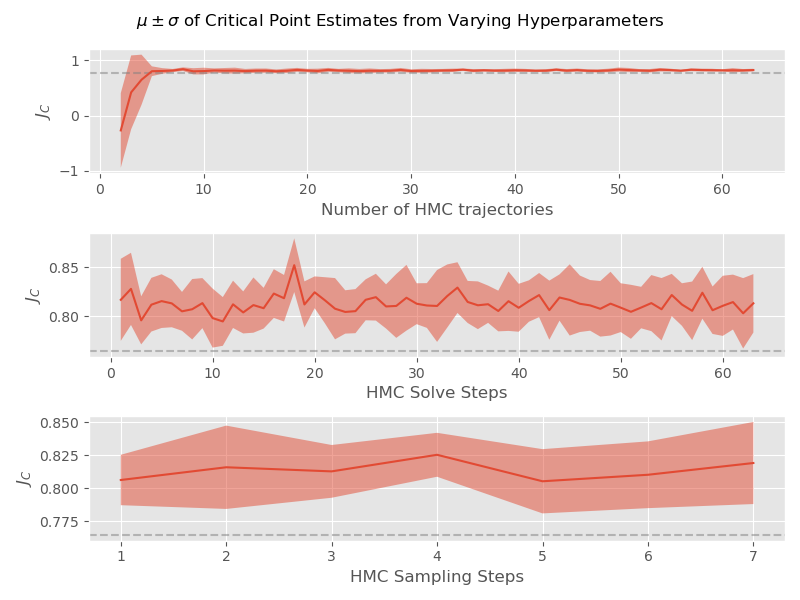
\includegraphics[width=0.45\textwidth]{tex/images/hmc-hyperparameters.png}
    \caption{\label{fig:hmc-hyperparameters}
        Hyperparameter space explorations for three HMC divergence hyperparameters. 
    }
\end{figure}

We conclude that:
\begin{itemize}
    \item The number of trajectories should be set above the minimal threshold to reduce heavy biasing error as well as variance. 
    \item The number of solve steps can be small. 
    \item The number of sampling steps can be small. 
\end{itemize}

\section{Conclusion}

In this work, we introduced the concept of real-space renormalization, presented the Ising model problem, and demonstrated how to apply real-space renormalization to it.
We then described a neural learning algorithm to approximate the renormalization group flow function over a Lieb lattice Ising model. 
We demonstrated its success at learning an accurate approximation, and observed its predictive abilities for critical points. 
We then discussed some aspects of the algorithmic design space, notably the reduction of bias via higher-dimensional representations, as well as the choice of loss function, whether to learn the flow or the monotone, and the role of sampler and contrastive divergence hyperparameters. 

All in all, the MLRG algorithm represents both a new way to automatically determine renormalization group flows, as well as an exciting new paradigm of machine learning. 
In the future, it will be interesting to see further research clarifying aspects such as flow versus monotone learning, the effect of contrastive approximations on the true gradient, and the significance of increasing the representational dimension.
There is also much follow-up work to do regarding applying this algorithm to other systems, such as different Ising models and maybe even non-Ising models as well as improving the algorithm to stably and efficiently handle higher-dimension representations. 

For reference, our implementations can be found at the repository https://github.com/jshe2304/dlrg. 

\bibliography{tex/references}

\end{document}